\documentclass{beamer}
\mode<presentation>
\usepackage{amsmath,amssymb,mathtools}
\usepackage{textcomp}
\usepackage{gensymb}
\usepackage{adjustbox}
\usepackage{subcaption}
\usepackage{enumitem}
\usepackage{multicol}
\usepackage{listings}
\usepackage{url}
\usepackage{graphicx} % <-- needed for images
\def\UrlBreaks{\do\/\do-}

\usetheme{Boadilla}
\usecolortheme{lily}
\setbeamertemplate{footline}{
  \leavevmode%
  \hbox{%
  \begin{beamercolorbox}[wd=\paperwidth,ht=2ex,dp=1ex,right]{author in head/foot}%
    \insertframenumber{} / \inserttotalframenumber\hspace*{2ex}
  \end{beamercolorbox}}%
  \vskip0pt%
}
\setbeamertemplate{navigation symbols}{}

\lstset{
  frame=single,
  breaklines=true,
  columns=fullflexible,
  basicstyle=\ttfamily\tiny   % tiny font so code fits
}

\numberwithin{equation}{section}

% ---- your macros ----
\providecommand{\nCr}[2]{\,^{#1}C_{#2}}
\providecommand{\nPr}[2]{\,^{#1}P_{#2}}
\providecommand{\mbf}{\mathbf}
\providecommand{\pr}[1]{\ensuremath{\Pr\left(#1\right)}}
\providecommand{\qfunc}[1]{\ensuremath{Q\left(#1\right)}}
\providecommand{\sbrak}[1]{\ensuremath{{}\left[#1\right]}}
\providecommand{\lsbrak}[1]{\ensuremath{{}\left[#1\right.}}
\providecommand{\rsbrak}[1]{\ensuremath{\left.#1\right]}}
\providecommand{\brak}[1]{\ensuremath{\left(#1\right)}}
\providecommand{\lbrak}[1]{\ensuremath{\left(#1\right.}}
\providecommand{\rbrak}[1]{\ensuremath{\left.#1\right)}}
\providecommand{\cbrak}[1]{\ensuremath{\left\{#1\right\}}}
\providecommand{\lcbrak}[1]{\ensuremath{\left\{#1\right.}}
\providecommand{\rcbrak}[1]{\ensuremath{\left.#1\right\}}}
\theoremstyle{remark}
\newtheorem{rem}{Remark}
\newcommand{\sgn}{\mathop{\mathrm{sgn}}}
\providecommand{\abs}[1]{\left\vert#1\right\vert}
\providecommand{\res}[1]{\Res\displaylimits_{#1}}
\providecommand{\norm}[1]{\lVert#1\rVert}
\providecommand{\mtx}[1]{\mathbf{#1}}
\providecommand{\mean}[1]{E\left[ #1 \right]}
\providecommand{\fourier}{\overset{\mathcal{F}}{ \rightleftharpoons}}
\providecommand{\system}{\overset{\mathcal{H}}{ \longleftrightarrow}}
\providecommand{\dec}[2]{\ensuremath{\overset{#1}{\underset{#2}{\gtrless}}}}
\newcommand{\myvec}[1]{\ensuremath{\begin{pmatrix}#1\end{pmatrix}}}
\newcommand{\mydet}[1]{\ensuremath{\begin{vmatrix}#1\end{vmatrix}}}

\newenvironment{amatrix}[1]{%
  \left(\begin{array}{@{}*{#1}{c}|*{#1}{c}@{}}
}{%
  \end{array}\right)
}

\newcommand{\myaugvec}[2]{\ensuremath{\begin{amatrix}{#1}#2\end{amatrix}}}
\let\vec\mathbf
% ---------------------

\title{Matgeo Presentation - Problem 12.693}
\author{ee25btech11056 - Suraj.N}

\begin{document}

\begin{frame}
  \titlepage
\end{frame}

\begin{frame}{Problem Statement}

Suppose the circles 

\begin{align*}
x^2 + y^2 + ax + 6 &= 0 \\
x^2 + y^2 + bx - 4 &= 0
\end{align*}
intersect each other orthogonally at the point $(1,2)$. Then $a+b = \_$

\end{frame}

\begin{frame}{Data}

\begin{table}[h!]
  \centering
  \begin{tabular}{|c|c|}
\hline
\textbf{Name} & \textbf{Value} \\ \hline
$\vec{A}$ & $\myvec{2 & 1 \\0 & 3}$ \\ \hline
\end{tabular}

  \caption*{Table : Circles and Point}
  \label{12.693}
\end{table}

\end{frame}

\begin{frame}{Solution}

The conic parameters for the two circles can be expressed as :

\begin{align}
  \vec{V_1} &= \vec{I} & \vec{u_1} &= \myvec{\tfrac{a}{2} \\0 } & f1 &= 6\\
  \vec{V_2} &= \vec{I} & \vec{u_2} &= \myvec{\tfrac{b}{2} \\ 0} & f2 &= -4
\end{align}

The point of intersection of the two circles is $\vec{P}$\\

The equation of tangent to Circle 1 at $\vec{P}$ is given as :

\begin{align}
  (\vec{V_1}\vec{P}+\vec{u_1})^\top\vec{x} + \vec{u_1}^\top\vec{P} + f_1 &= 0 & \vec{n_1} &= \vec{V_1}\vec{P}+\vec{u_1} 
\end{align}

The equation of tangent to Circle 2 at $\vec{P}$ is given as :

\begin{align}
  (\vec{V_2}\vec{P}+\vec{u_2})^\top\vec{x} + \vec{u_2}^\top\vec{P} + f_2 &= 0 & \vec{n_2} &= \vec{V_2}\vec{P}+\vec{u_2} 
\end{align}

\end{frame}

\begin{frame}{Solution}

As the tangents at $\vec{P}$ are perpendicular , the normal vectors of the tangents are also perpendicular 

\begin{align}
  \vec{n_1}^\top\vec{n_2} = 0\\
  (\vec{V_1}\vec{P}+\vec{u_1})^\top(\vec{V_2}\vec{P}+\vec{u_2}) = 0\\
  (\vec{P}+\vec{u_1})^\top(\vec{P}+\vec{u_2}) = 0\\
  (\vec{P}^\top+\vec{u_1}^\top)(\vec{P}+\vec{u_2}) = 0 \label{eq:tangent} \\
  \myvec{\tfrac{a+2}{2} & 2}\myvec{\tfrac{b+2}{2}\\2} = 0\\
  2(a+b) + ab + 20 = 0  \label{eq:a+b} 
\end{align}

As $\vec{P}$ lies on both the circles we get :

\begin{align}
  \vec{P}^\top \vec{P} + 2\vec{u_1}^\top \vec{P} + f_1 = 0 \label{eq:circle1} \\
  \vec{P}^\top \vec{P} + 2\vec{u_2}^\top \vec{P} + f_2 = 0 
\end{align}

\end{frame}

\begin{frame}{Solution}

By subtracting the above two equations we get :

\begin{align}
  (\vec{u_1}^\top - \vec{u_2}^\top)\vec{P} = \frac{f_2 - f_1}{2} \label{eq:p1} 
\end{align}

If we substitue \eqref{eq:circle1} in \eqref{eq:tangent} we get :

\begin{align}
  (\vec{u_2}^\top - \vec{u_1}^\top)\vec{P} + \vec{u_1}^\top\vec{u_2} - f_1 = 0\\
  (\vec{u_1}^\top - \vec{u_2}^\top)\vec{P} = \vec{u_1}^\top\vec{u_2} - f_1   \label{eq:p2} 
\end{align}

From \eqref{eq:p1} and \eqref{eq:p2} , we get :

\begin{align}
  \vec{u_1}^\top\vec{u_2} = \frac{f_1+f_2}{2}\\
  ab = 4  \label{eq:ab}
\end{align}

\end{frame}

\begin{frame}{Solution}

By substituting \eqref{eq:ab} in \eqref{eq:a+b} , we get :

\begin{align}
a + b = -12
\end{align}

\end{frame}

\begin{frame}{Plot}

\begin{figure}[h!]
  \centering
  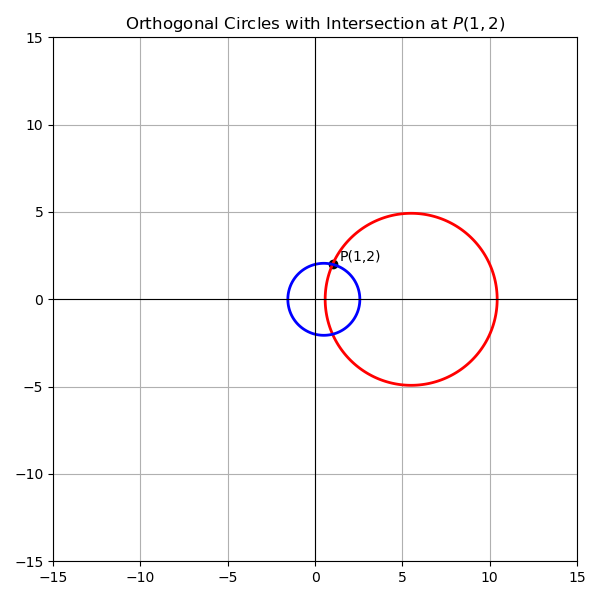
\includegraphics[width=0.6\columnwidth]{figs/circles.png} 
   \caption*{Fig : Circles}
  \label{Fig1}
\end{figure}

\end{frame}


\end{document}
